\documentclass[compress,handout]{beamer}
\mode<presentation>
{
 \usetheme{Vilanova}
}

\usepackage[french]{babel}

\usepackage[utf8]{inputenc}

\usepackage{times}
\usepackage[T1]{fontenc}

\usepackage{amsfonts}
\usepackage{amsmath}
\usepackage{amssymb}
\usepackage{tikz}
\usepackage{eurosym}
%\usepackage{url}
\usepackage[normal]{subfigure}
\newcommand{\goodgap}{%
	\hspace{\subfigtopskip}%
	\hspace{\subfigbottomskip}}



%\newtheorem{definition}{Definition}

\title{Traitement d'images de télédétection}
\subtitle{Extraction de primitives}




\author
{jordi.inglada@cesbio.cnes.fr}
\normalsize

\institute[Cesbio] % (optional, but mostly needed)
{\textsc{Centre d'Études Spatiales de la Biosphère, Toulouse, France}}

\date{}

\pgfdeclareimage[height=96mm,width=128mm]{background}{fondsClairSansLogo}
\setbeamertemplate{background}{\pgfuseimage{background}}
\pgfdeclareimage[height=0.6cm]{logoIncrust}{logoIncrust}
\pgfdeclareimage[height=0.5cm]{logo_cesbio}{logo_cesbio}
\logo{
\begin{tabular}{lp{0.25\textwidth}lp{0.25\textwidth}r}
\href{http://www.cesbio.ups-tlse.fr/}{\pgfuseimage{logo_cesbio}}
&&\footnotesize{AUF - Marrakech 2011}&&
\href{http://www.orfeo-toolbox.org}{\pgfuseimage{logoIncrust}}\\
\end{tabular}
}


\subject{Extraction de primitives}




% Delete this, if you do not want the table of contents to pop up at
% the beginning of each subsection:
\AtBeginSubsection[]
{
  \begin{frame}<beamer>
    \frametitle{Outline}
    \tableofcontents[currentsection,currentsubsection]
  \end{frame}
}




% If you wish to uncover everything in a step-wise fashion, uncomment
% the following command: 

%\beamerdefaultoverlayspecification{<+->}
\begin{document}

\begin{frame}
  \titlepage
  \begin{center}
{\tiny Ce contenu est dérivé de la formation \href{http://www.orfeo-toolbox.org/packages/PragmaticRemoteSensing-handout.pdf}{``Pragmatic Remote
  Sensing''} dispensée par J. Inglada et E. Christophe en juillet 2010
  dans le cadre du colloque IGARSS. Il est mis à disposition selon les termes de la licence :\\
Creative Commons Paternité – Partage à l’Identique 3.0 non transcrit.} \href{http://creativecommons.org/licenses/by-sa/3.0/}{
\includegraphics[width=0.05\textwidth]{/home/inglada/Dev/GH/IGARSS2010/Tutorial/Slides/Ressources/CC-licence.png}}    
  \end{center}
\end{frame}

\section{Introduction}

\begin{frame}
\frametitle{Primitives}

\begin{block}{Connaissance a priori}
\begin{itemize}
\item Les primitives constituent une façon simple d'introduire de la
  connaissance a priori sur le contenu des images
\item Familles de primitives : radiométriques, textures,\ldots
\item Construction de primitives sur mesure pour une application donnée
\end{itemize}
\end{block}

\end{frame}

\section{Radiométrie}

\begin{frame}
\frametitle{Indices radiométriques}
Indice de végétation NDVI: Normalized Difference Vegetation Index \cite{Rouse1973-NDVI}

\begin{equation}
 \mathbf{NDVI} = \frac{L_{NIR}-L_{r}}{L_{NIR}+L_{r}}
 \end{equation}

\begin{thebibliography}{noidea}
\footnotesize
\bibitem{Rouse1973-NDVI}
J. W. Rouse. ``Monitoring the vernal advancement and retrogradation of natural vegetation,''{\em Type ii report, NASA/GSFCT, Greenbelt, MD, USA}, 1973. 12.1.1
\end{thebibliography}

\end{frame}

\begin{frame}
\frametitle{Indices de végétation 1/3}
\footnotesize  \centering
\begin{tabular}{|c|l|}
\hline
RVI &  Ratio Vegetation Index \cite{Pearson1972-RVI}\\
PVI & Perpendicular Vegetation Index \cite{Richardson1977-PVI,Wiegand1991-PVI}\\ 
SAVI & Soil Adjusted Vegetation Index \cite{Huete1988-SAVI} \\
TSAVI & Transformed Soil Adjusted Vegetation Index \cite{Baret1989-TSAVI,Baret1991-TSAVI} \\
\hline
\end{tabular}
\begin{thebibliography}{noidea}
\tiny
\bibitem{Pearson1972-RVI}
R.~L. Pearson and L.~D. Miller. Remote mapping of standing crop biomass for estimation of the
  productivity of the shortgrass prairie, pawnee national grasslands,
        colorado.  In {\em Proceedings of the 8th International Symposium on Remote
  Sensing of the Environment II}, pages 1355--1379, 1972.
\bibitem{Richardson1977-PVI}
A.~J. Richardson and C.~L. Wiegand.
 Distinguishing vegetation from soil background information.
 {\em Photogrammetric Engineering and Remote Sensing},
  43(12):1541--1552, 1977.
\bibitem{Wiegand1991-PVI}
C.~L. Wiegand, A.~J. Richardson, D.~E. Escobar, and A.~H. Gerbermann.
 Vegetation indices in crop assessments.
 {\em Remote Sensing of Environment}, 35:105--119, 1991.
\bibitem{Huete1988-SAVI}
A.~R. Huete.
 A soil-adjusted vegetation index ({SAVI}).
 {\em Remote Sensing of Environment}, 25:295--309, 1988.
\bibitem{Baret1991-TSAVI}
E.~Baret and G.~Guyot.
 Potentials and limits of vegetation indices for {LAI} and {APAR}
  assessment.
 {\em Remote Sensing of Environment}, 35:161--173, 1991.

\bibitem{Baret1989-TSAVI}
E.~Baret, G.~Guyot, and D.~J. Major.
 {TSAVI}: A vegetation index which minimizes soil brightness effects
  on {LAI} and {APAR} estimation.
 In {\em Proceedings of the 12th Canadian Symposium on Remote Sensing,
  Vancouver, Canada}, pages 1355--1358, 1989.
\end{thebibliography}
\end{frame}

\begin{frame}
\frametitle{Indices de végétation 2/3}
\footnotesize \centering
\begin{tabular}{|c|l|}
\hline
MSAVI & Modified Soil Adjusted Vegetation Index  \cite{Qi1994-MSAVI} \\
MSAVI2 & Modified Soil Adjusted Vegetation Index  \cite{Qi1994-MSAVI} \\
GEMI &   Global Environment Monitoring Index \cite{Pinty1992-GEMI} \\
WDVI & Weighted Difference Vegetation Index  \cite{Clevers1988-WDVI,Clevers1991-WDVI} \\ 
AVI & Angular Vegetation Index  \cite{AVI}\\
\hline
\end{tabular}
\begin{thebibliography}{noidea}
\tiny
\bibitem{Qi1994-MSAVI}
J.~Qi, A.~. Chehbouni, A.~Huete, Y.~Kerr, and S.~Sorooshian.
 A modified soil adjusted vegetation index.
 {\em Remote Sensing of Environment}, 47:1--25, 1994.
\bibitem{Pinty1992-GEMI}
B.~Pinty and M.~M. Verstraete.
 {GEMI}: a non-linear index to monitor global vegetation from
  satellites.
 {\em Vegetatio}, 101:15--20, 1992.
\bibitem{Clevers1988-WDVI}
J.~Clevers.
 The derivation of a simplified reflectance model for the estimation
  of leaf area index.
 {\em Remote Sensing of Environment}, 25:53--69, 1988.

\bibitem{Clevers1991-WDVI}
J.~Clevers.
 Application of the wdvi in estimating lai at the generative stage of
  barley.
 {\em ISPRS Journal of Photogrammetry and Remote Sensing},
  46(1):37--47, 1991.
\bibitem{AVI}
S.~Plummer, P.~North, and S.~Briggs.
 {The Angular Vegetation Index (AVI): an atmospherically resistant
  index for the Second Along-Track Scanning Radiometer (ATSR-2)}.
 In {\em Sixth International Symposium on Physical Measurements and
  Spectral Signatures in Remote Sensing, Val d'Isere}, 1994.
\end{thebibliography}
\end{frame}

\begin{frame}
\frametitle{Indices de végétation 3/3}
\footnotesize \centering
\begin{tabular}{|c|l|}
\hline
ARVI & Atmospherically Resistant  Vegetation Index \cite{ARVI} \\
TSARVI & Transformed Soil Adjusted Vegetation Index   \cite{ARVI} \\
EVI & Enhanced Vegetation Index \cite{Huete1994-EVI,Justice1998-EVI} \\
IPVI & Infrared Percentage Vegetation Index  \cite{Crippen1990-IPVI} \\
TNDVI & Transformed NDVI  \cite{Deering1975-TNDVI} \\
\hline
\end{tabular}
\begin{thebibliography}{noidea}
\tiny
\bibitem{ARVI}
Y.~J. Kaufman and D.~Tanr\'e.
 {Atmospherically Resistant Vegetation Index (ARVI) for EOS-MODIS}.
 {\em Transactions on Geoscience and Remote Sensing}, 40(2):261--270,
  Mar. 1992.
\bibitem{Huete1994-EVI}
A.~R. Huete, C.~Justice, and H.~Liu.
 Development of vegetation and soil indices for {MODIS-EOS}.
 {\em Remote Sensing of Environment}, 49:224--234, 1994.
\bibitem{Justice1998-EVI}
C.~O. Justice, et al.
 The moderate resolution imaging spectroradiometer ({MODIS}): Land
  remote sensing for global change research.
 {\em IEEE Transactions on Geoscience and Remote Sensing}, 36:1--22,
  1998.
\bibitem{Crippen1990-IPVI}
R.~E. Crippen.
 Calculating the vegetation index faster.
 {\em Remote Sensing of Environment}, 34(1):71--73, 1990.
\bibitem{Deering1975-TNDVI}
D.~W. Deering, J.~W. Rouse, R.~H. Haas, and H.~H. Schell.
 Measuring \"forage production\" of grazing units from {L}andsat-{MSS}
  data.
 In {\em Proceedings of the Tenth International Symposium on Remote
  Sensing of the Environment. ERIM, Ann Arbor, Michigan, USA}, pages
  1169--1198, 1975.
\end{thebibliography}
\end{frame}

\begin{frame}
\frametitle{Exemple: NDVI}
\begin{columns}
\begin{column}{0.5\textwidth}
\begin{figure}[]
  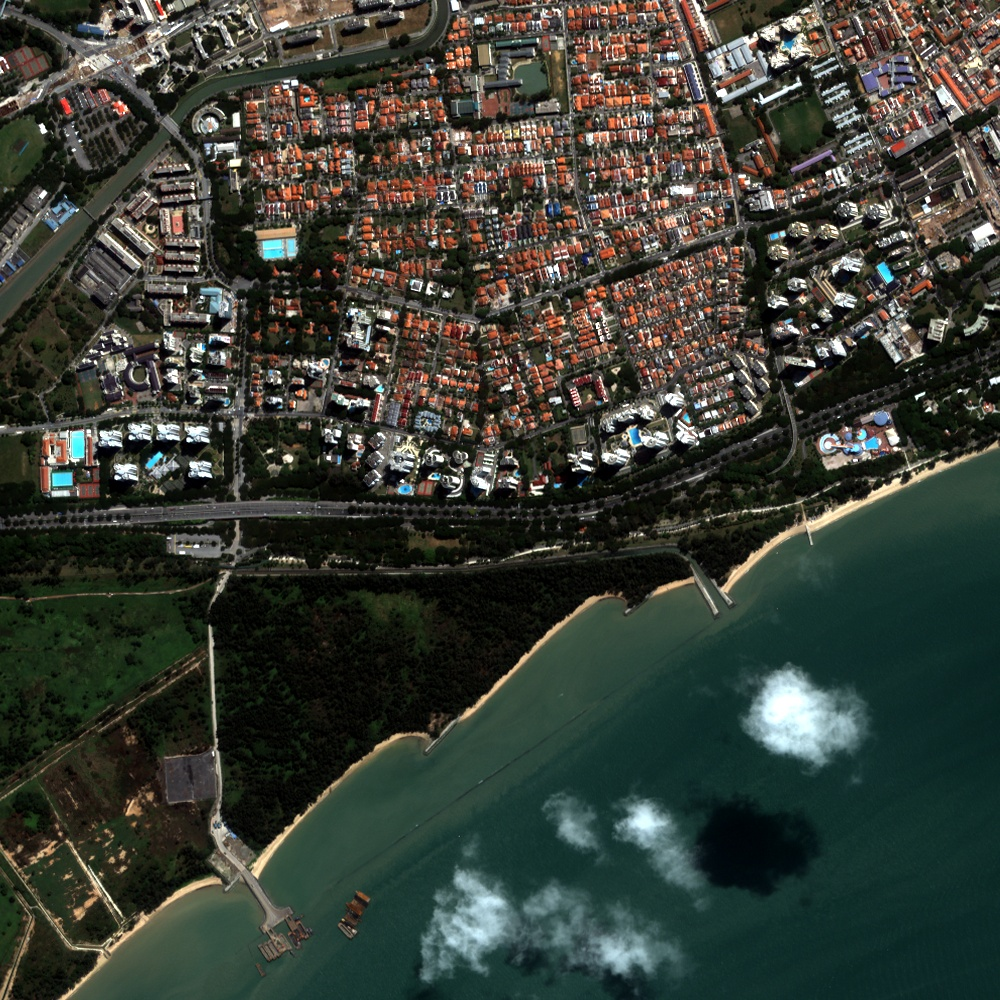
\includegraphics[width=1.0\textwidth]{radio2-extract-3b.jpg}
\end{figure}
\end{column}
\begin{column}{0.5\textwidth}
\begin{figure}[]
  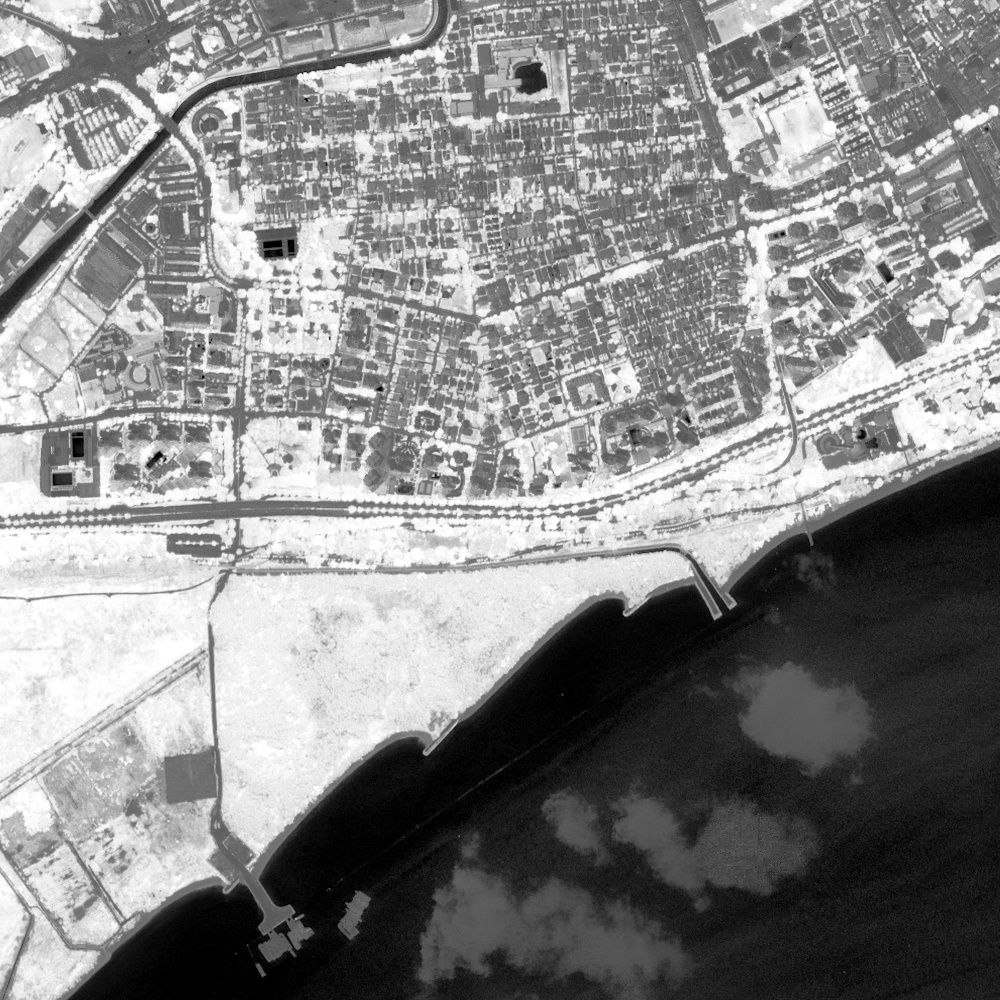
\includegraphics[width=1.0\textwidth]{Radiometry-NDVI.jpg}
\end{figure}
\end{column}
\end{columns}
\end{frame}


\begin{frame}
\frametitle{Indices de sol}
\footnotesize \centering
\begin{tabular}{|c|l|}
\hline
IR  & Redness Index  \cite{Pouget1990-IRIC} \\
IC  & Color Index  \cite{Pouget1990-IRIC} \\
IB  & Brilliance Index  \cite{Nicoloyanni1990-IB} \\
IB2 & Brilliance Index  \cite{Nicoloyanni1990-IB} \\
\hline
\end{tabular}
\begin{thebibliography}{noidea}
\tiny
\bibitem{Pouget1990-IRIC}
P.~et~al.
 Caractéristiques spectrales des surfaces sableuses de la région
  côtière nord-ouest de l'{E}gypte: application aux données satellitaires
  {S}pot.
 In {\em 2ème Journées de Télédétection: Caractérisation et suivi des
  milieux terrestres en régions arides et tropicales}, pages 27--38. ORSTOM,
  Collection Colloques et Séminaires, Paris, Dec. 1990.
\bibitem{Nicoloyanni1990-IB}
E.~Nicoloyanni.
 Un indice de changement diachronique appliqu\'e deux sc\`enes
  {L}andsat {MSS} sur {A}th\`enes (gr\`ece).
 {\em International Journal of Remote Sensing}, 11(9):1617--1623,
  1990.
\end{thebibliography}
\end{frame}

\begin{frame}
\frametitle{Exemple: IC}
\begin{columns}
\begin{column}{0.5\textwidth}
\begin{figure}[]
  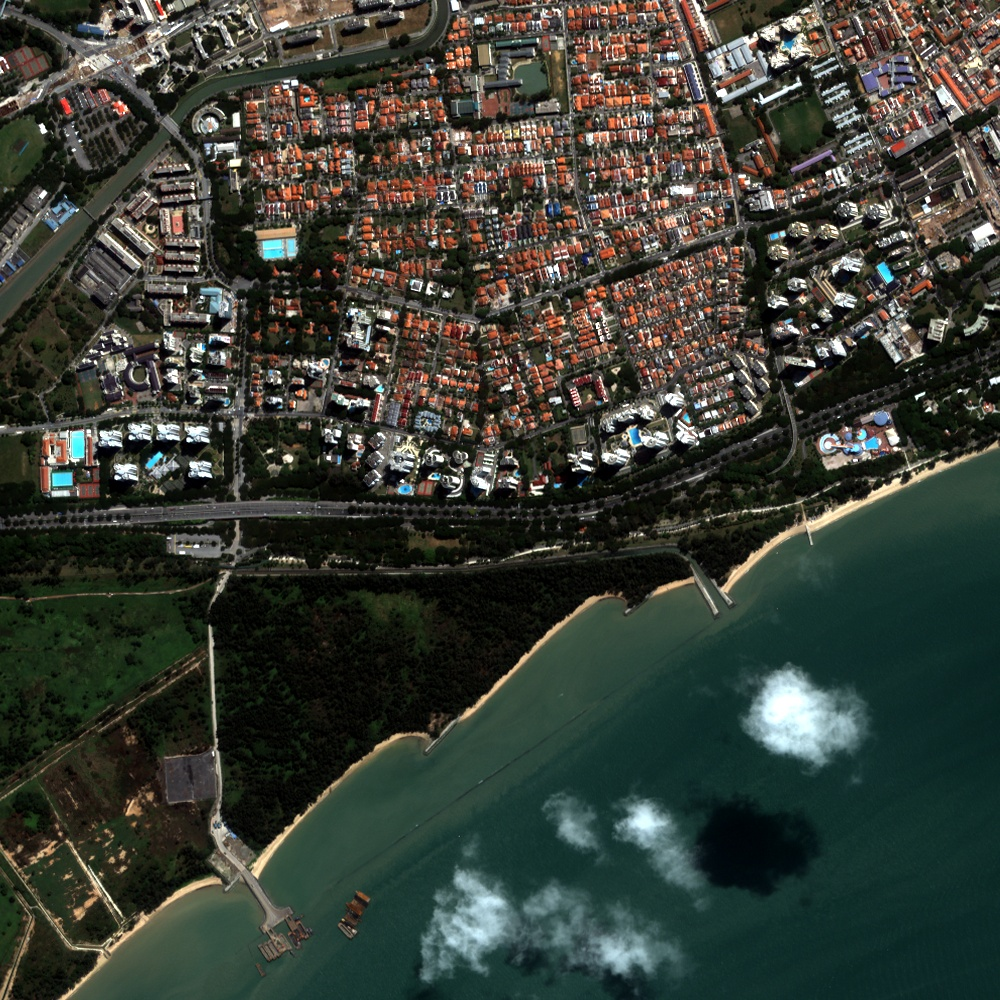
\includegraphics[width=1.0\textwidth]{radio2-extract-3b.jpg}
\end{figure}
\end{column}
\begin{column}{0.5\textwidth}
\begin{figure}[]
  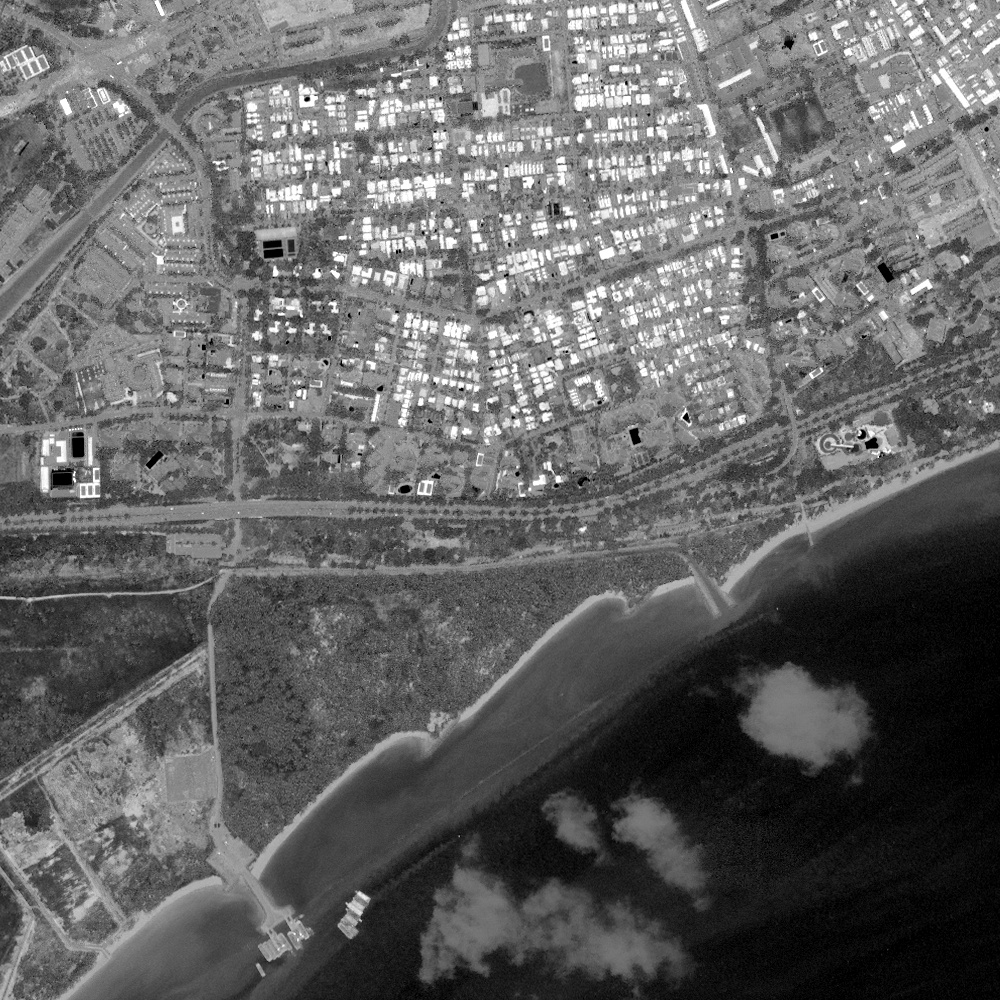
\includegraphics[width=1.0\textwidth]{Radiometry-IC.jpg}
\end{figure}
\end{column}
\end{columns}
\end{frame}


\begin{frame}
\frametitle{Indices d'eau}
\footnotesize \centering
\begin{tabular}{|c|l|}
\hline
SRWI & Simple Ratio Water Index \cite{ZarcoTejada2001-SRWI} \\
NDWI & Normalized Difference Water Index  \cite{Gao1996-NDWI} \\
NDWI2 &  Normalized Difference Water Index \cite{McFeeters1996-NDWI2} \\
MNDWI &  Modified Normalized Difference Water Index  \cite{Xu2006-MNDWI} \\
NDPI &  Normalized Difference Pond Index \cite{Lacaux2007-NDTI} \\
NDTI &  Normalized Difference Turbidity Index  \cite{Lacaux2007-NDTI} \\
SA & Spectral Angle \\
\hline
\end{tabular}
\begin{thebibliography}{noidea}
\tiny
\bibitem{ZarcoTejada2001-SRWI}
P.~J. Zarco-Tejada and S.~Ustin.
 Modeling canopy water content for carbon estimates from {MODIS} data
  at land {EOS} validation sites.
 In {\em International Geoscience and Remote Sensing Symposium, IGARSS
  '01}, pages 342--344, 2001.
\bibitem{Gao1996-NDWI}
B.~cai Gao.
 {NDWI} - a normalized difference water index for remote sensing of
  vegetation liquid water from space.
 {\em Remote Sensing of Environment}, 58(3):257--266,
        Dec. 1996.
\bibitem{McFeeters1996-NDWI2}
S.~K. McFeeters.
 The use of the normalized difference water index ({NDWI}) in the
  delineation of open water features.
 {\em International Journal of Remote Sensing}, 17(7):1425--1432,
  1996.
\bibitem{Xu2006-MNDWI}
H.~Xu.
 Modification of normalised difference water index (ndwi) to enhance
  open water features in remotely sensed imagery.
 {\em International Journal of Remote Sensing}, 27(14):3025--3033,
  2006.
\bibitem{Lacaux2007-NDTI}
J.~Lacauxa, Y.~T. andC. Vignollesa, J.~Ndioneb, and M.~Lafayec.
 Classification of ponds from high-spatial resolution remote sensing:
  Application to rift valley fever epidemics in Senegal.
 {\em Remote Sensing of Environment}, 106(1):66--74, 2007.
\end{thebibliography}
\end{frame}

\begin{frame}
\frametitle{Exemple: NDWI2}
\begin{columns}
\begin{column}{0.5\textwidth}
\begin{figure}[]
  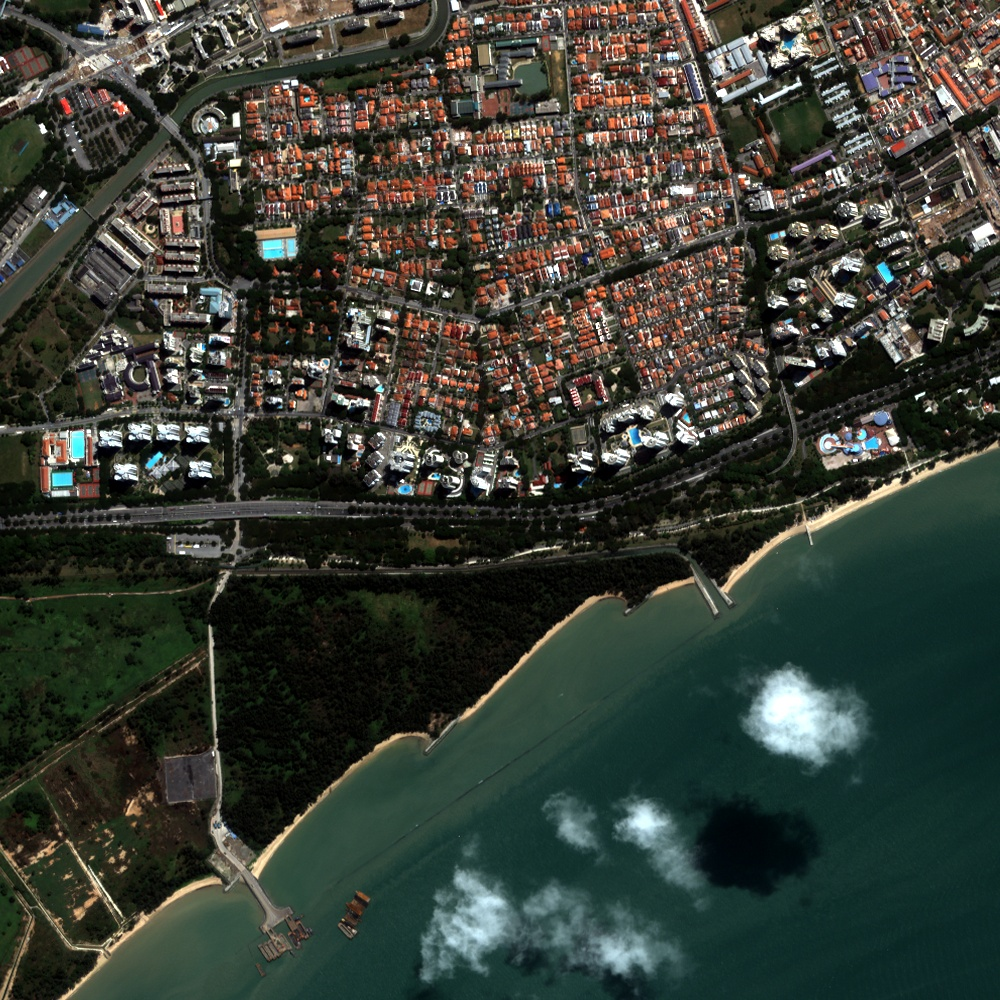
\includegraphics[width=1.0\textwidth]{radio2-extract-3b.jpg}
\end{figure}
\end{column}
\begin{column}{0.5\textwidth}
\begin{figure}[]
  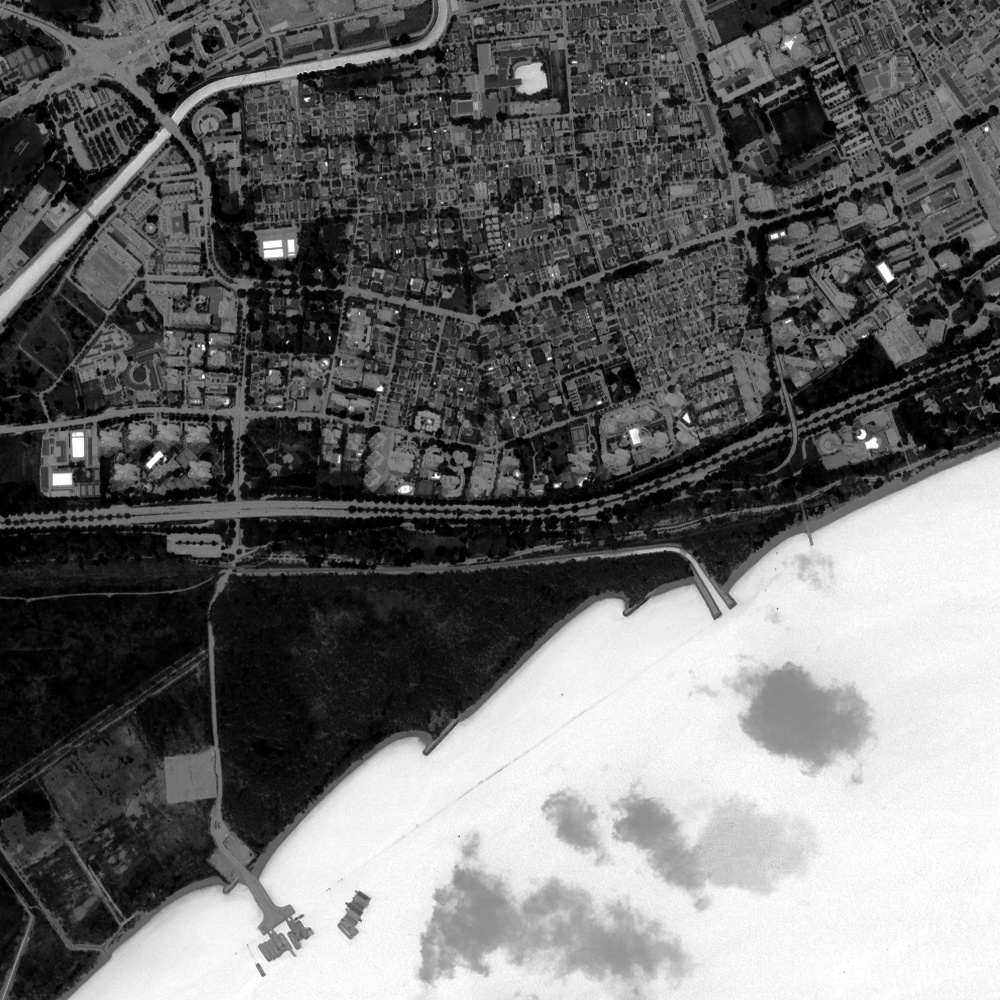
\includegraphics[width=1.0\textwidth]{Radiometry-NDWI2.jpg}
\end{figure}
\end{column}
\end{columns}
\end{frame}


\begin{frame}
\frametitle{Indices de bâti}
\footnotesize \centering
\begin{tabular}{|c|l|}
\hline
NDBI &  Normalized Difference Built Up Index \cite{Zha2003-NDBI} \\
ISU &  Indice de Surfaces Bâties \cite{Abdellaoui1997-ISU} \\
\hline
\end{tabular}
\begin{thebibliography}{noidea}
\tiny
\bibitem{Zha2003-NDBI}
Y.~Z. J. G.~S. Ni.
 Use of normalized difference built-up index in automatically mapping
  urban areas from {TM} imagery.
 {\em International Journal of Remote Sensing}, 24(3):583--594,
        2003.
\bibitem{Abdellaoui1997-ISU}
A.~Abdellaoui and A.~Rougab.
 Caract\'erisation de la réponse du b\^ati: application au complexe
  urbain de {B}lida ({A}lg\'erie).
 In {\em T\'el\'ed\'etection des milieux urbains et p\'eriurbains,
  AUPELF - UREF, Actes des sixi\`emes Journ\'ees scientifiques du r\'eseau
  T\'el\'ed\'etection de l'AUF}, pages 47--64, 1997.
\end{thebibliography}
\end{frame}


\section{Textures}

\begin{frame}
\frametitle{Texture}
\tiny \centering
\begin{tabular}{cc}
& \\
Énergie & $ f_1 = \sum_{i,j}g(i, j)^2 $ \\
& \\
& \\
Entropie & $ f_2 = -\sum_{i,j}g(i, j) \log_2 g(i, j)$, or 0 if $g(i, j) = 0$ \\
& \\
& \\
Corrélation & $ f_3 = \sum_{i,j}\frac{(i - \mu)(j - \mu)g(i, j)}{\sigma^2} $ \\
& \\
& \\
Moment de Différence&  $f_4 = \sum_{i,j}\frac{1}{1 + (i - j)^2}g(i, j) $ \\
& \\
& \\
Inertie (Contraste) & $ f_5 = \sum_{i,j}(i - j)^2g(i, j) $ \\
& \\
& \\
Cluster Shade & $ f_6 = \sum_{i,j}((i - \mu) + (j - \mu))^3 g(i, j) $ \\
& \\
Cluster Prominence & $ f_7 = \sum_{i,j}((i - \mu) + (j - \mu))^4 g(i, j) $ \\
& \\
& \\
Corrélation de Haralick& $ f_8 = \frac{\sum_{i,j}(i, j) g(i, j) -\mu_t^2}{\sigma_t^2} $ \\
& \\
\end{tabular}
\begin{thebibliography}{noidea}
\tiny
\bibitem{Haralick1973}
Robert~M. Haralick, K.~Shanmugam, and Its'Hak Dinstein,
 ``Textural features for image classification,''
 {\em IEEE Transactions on Systems, Man and Cybernetics}, vol. 3, no.
  6, pp. 610--621, Nov 1973.
\end{thebibliography}
\end{frame}


\begin{frame}
\frametitle{Exemple: Inertie sur la bande verte}
\begin{columns}
\begin{column}{0.5\textwidth}
\begin{figure}[]
  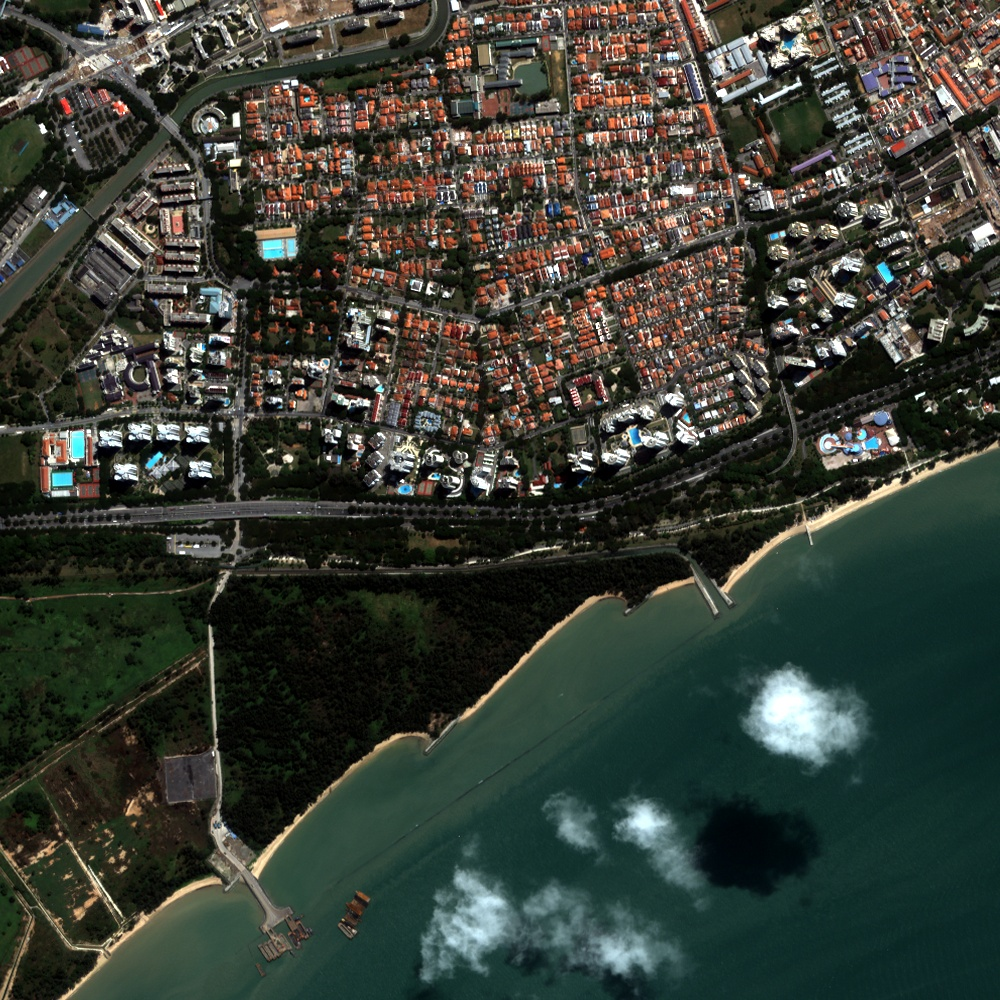
\includegraphics[width=1.0\textwidth]{radio2-extract-3b.jpg}
\end{figure}
\end{column}
\begin{column}{0.5\textwidth}
\begin{figure}[]
  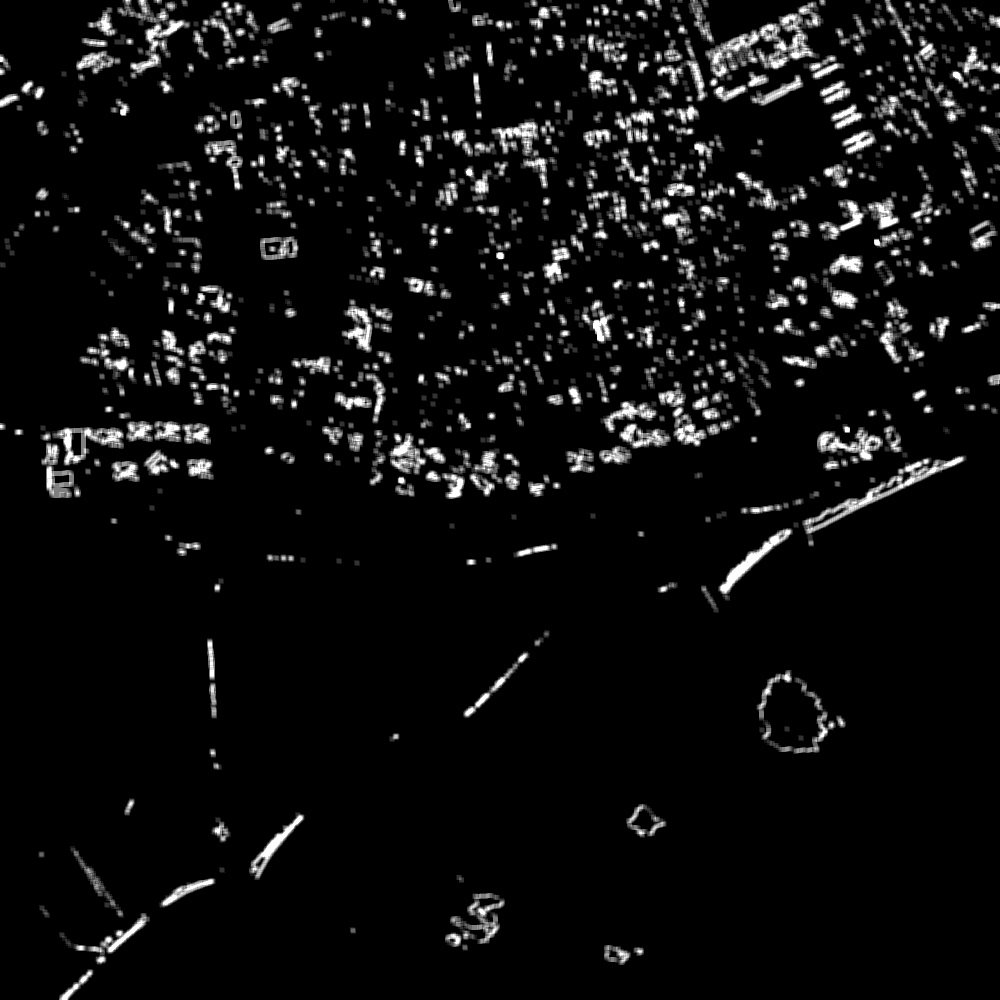
\includegraphics[width=1.0\textwidth]{Texture-Inertia-R2-2-O1-1-C1.jpg}
\end{figure}
\end{column}
\end{columns}
\end{frame}


\section{Autres}


\begin{frame}
\frametitle{Combinaison de primitives}
Exemple: distance à l'eau
\begin{columns}
\begin{column}{0.32\textwidth}
\begin{figure}[]
  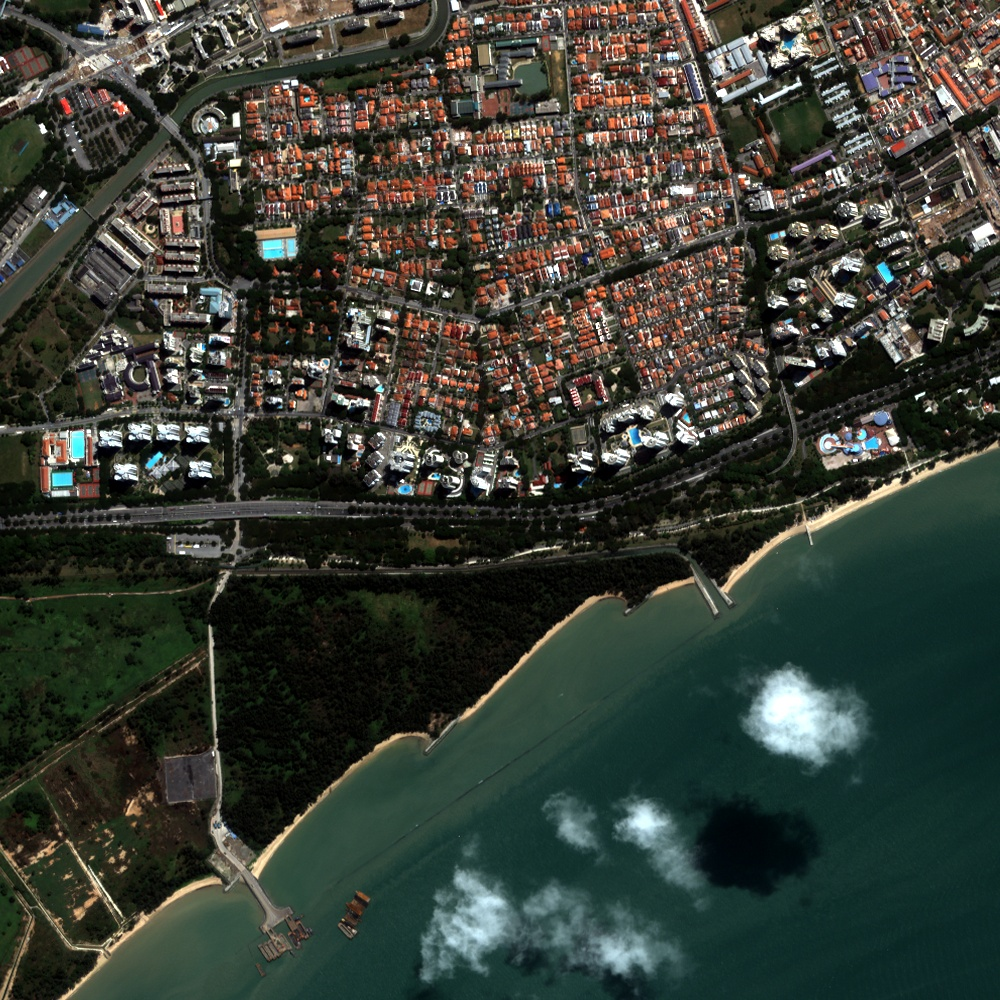
\includegraphics[width=1.0\textwidth]{radio2-extract-3b.jpg}
\end{figure}
\end{column}
\begin{column}{0.32\textwidth}
\begin{figure}[]
  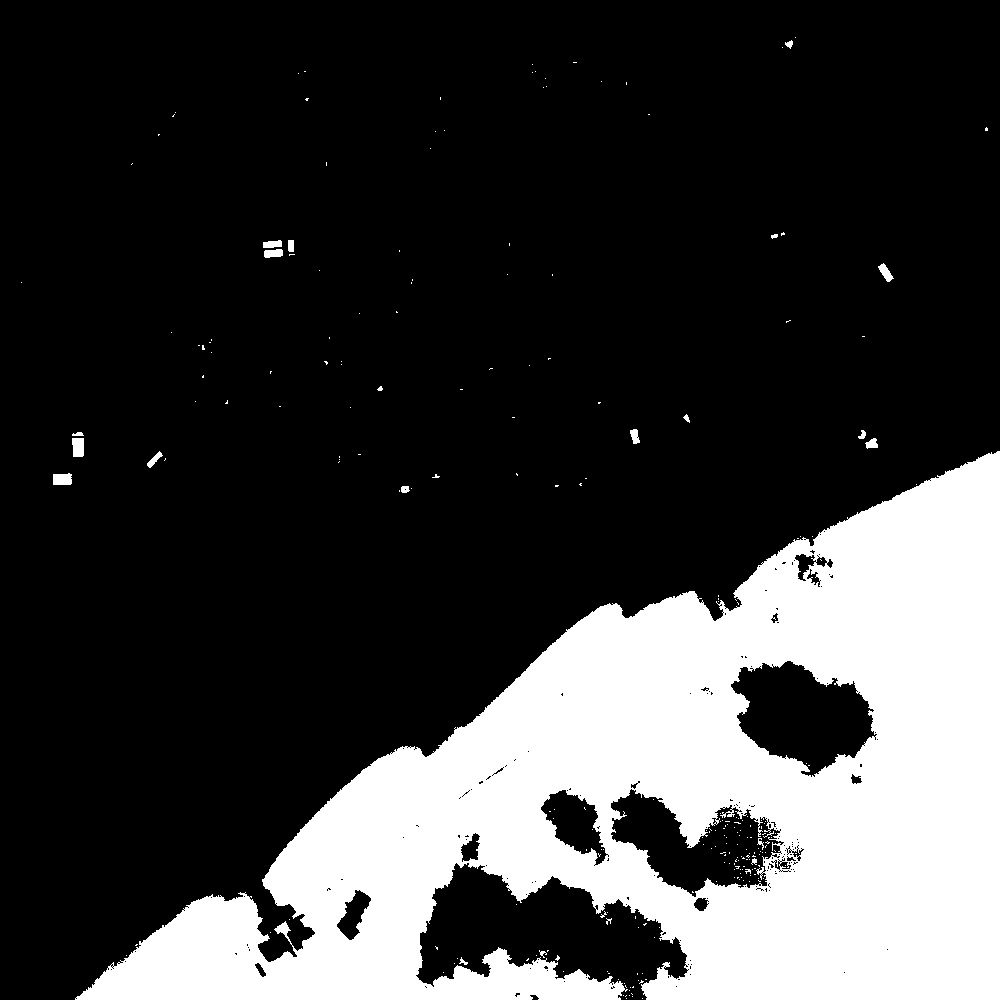
\includegraphics[width=1.0\textwidth]{MNDWI2-threshold.jpg}
\end{figure}
\end{column}
\begin{column}{0.32\textwidth}
\begin{figure}[]
  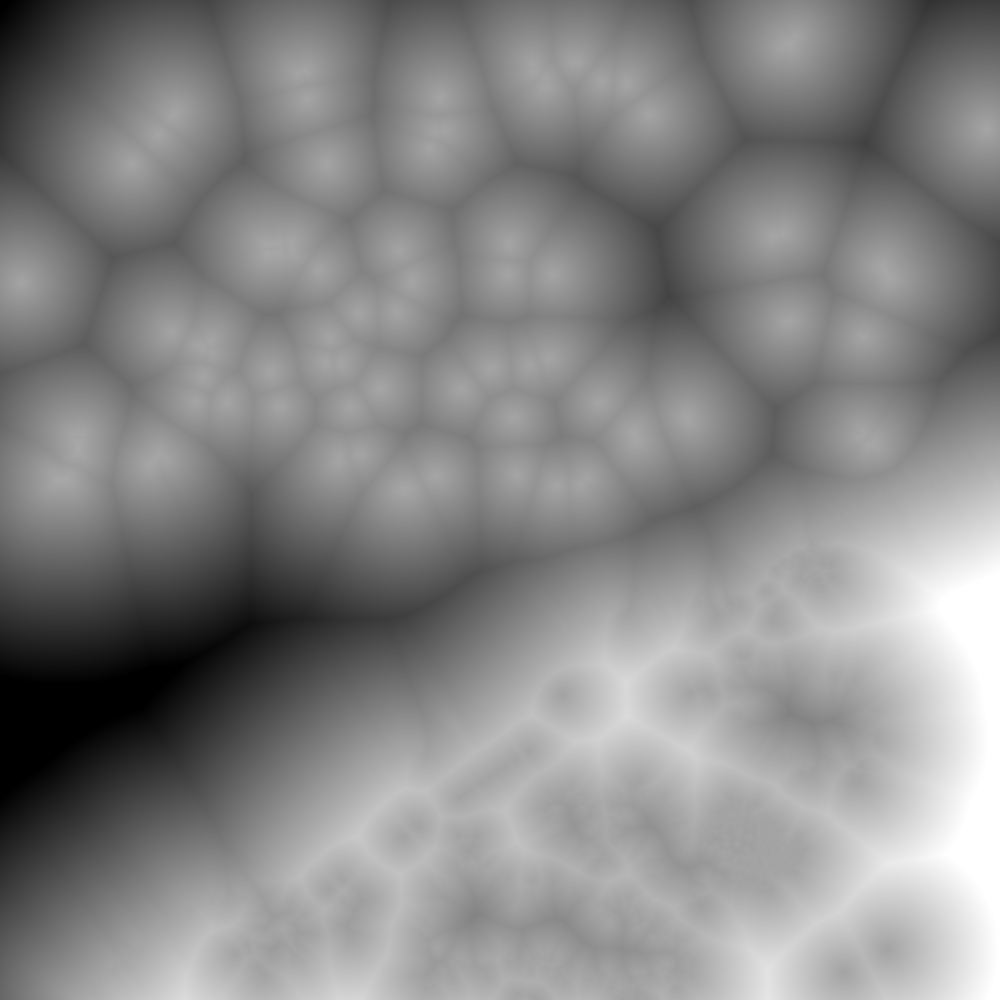
\includegraphics[width=1.0\textwidth]{DistanceFromWater.jpg}
\end{figure}
\end{column}
\end{columns}
\end{frame}


\begin{frame}
\frametitle{La main à la pâte}
\begin{enumerate}
\item Monteverdi: Filtering $\rightarrow$ Feature extraction
\item Choisir une image
  \begin{itemize}
  \item /home/auf/OTB/Data/Examples/qb\_RoadExtract.tif
  \end{itemize}
\item Choisir une primitive
\item Essayer différents paramètres et regarder les résultats
\item Utiliser l'onglet ``output'' pour sélectionner les primitives utiles
\item Générer l'image de primitives
\end{enumerate}

\end{frame}

\end{document}
